\chapter{TVN: Electrical stimulation}
\label{chap:Stim}
\tvnnote{Torbjoern skriver dette}

\section{\red{TVN TO WRITE THIS}}
\begin{itemize}
\item General principle with illustration figure?
\item Only change in external potential matters, emphasizing importance of distance to electrode and electrode size.
\item Only change along neurites matter, not across membrane (electric field across membrane is already immense).
\item Activation function: Strengths and weaknesses
\item Axon terminals are main targets of action potential initiation, seen both in experiments and simulations.
\item Negative current pulses will depolarize proximal part of cell and hyperpolarize distal part of cell. Opposite for positive current.
\end{itemize}

\section{Mathematical investigation of toy example}
\tvnnote{Konvensjonene her er ikke helt i sync med tidligere kapitler.}
Extracellular injection of currents can cause strong extracellular potentials that affects neurons. However, getting an intuitive understanding of what is happening can be hard. We therefore mathematically explore a toy example, consisting of a two-compartment neuron model, being stimulated by a single extracellular current source, $I_{EC}$ (Fig.~\ref{Stim:fig:two_comp}). 

\begin{figure}[!ht]
\begin{center}
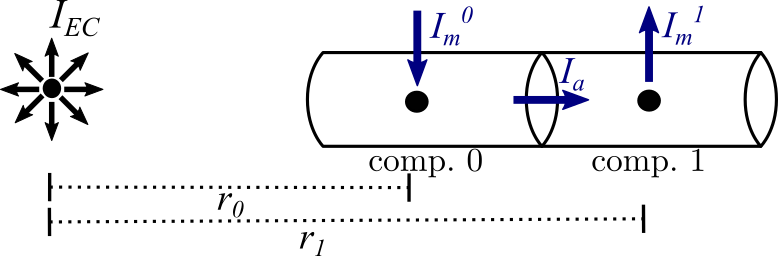
\includegraphics[width=0.5\textwidth]{Figures/Stim/ext_stim_two_comp.png}
\end{center}
\caption{\textbf{Two-compartment toy example.} 
}
\label{Stim:fig:two_comp}
\end{figure}

%This derivation closely mimics \cite**{Tveito2017}.
The transmembrane currents from either of the two neural compartment, $k$, can be written (sec \ref{sec:Neuron:membranecurrents}),
\begin{equation}
I_m^k = I^k_c + I^k_{ion},
\end{equation}
where $I_c^k$ and $I_{ion}^k$ are the capacitive and ionic current of compartment $k$, respectively.
The axial current, $I^a$, between compartment 0 and 1 is found by applying Ohm's law (Eq. \ref{Neuron:eq:axialcurrents}),
\begin{equation}
I_a = \frac{u_i^0 - u_i^1}{4 R_a L / (\pi d^2)}
\end{equation}
where $u_i^k$ is the intracellular potential. The membrane potential is defined as the difference between the intracellular and extracellular potential, $V_m = u_i - u_e$, and we can therefore write
\begin{equation}
I_a = \frac{-\Delta V_m - \Delta u_e}{4 R_a L / (\pi d^2)},
\end{equation}
where $\Delta V_m = V_m^1 - V_m^0$ and $\Delta u_e = u_e^1 - u_e^0$.
 
 
From current conservation, we know that the current flowing out of a compartment must equal the current flowing into the compartment, implying the relations (defining a positive axial current as going from compartment 0 to compartment 1),
\begin{eqnarray}
I_m^0 &=& - I_a = \frac{\Delta V_m + \Delta u_e}{4 R_a L / (\pi d^2)} \\
I_m^1 &=& + I_a =  \frac{-\Delta V_m - \Delta u_e}{4 R_a L / (\pi d^2)}.
\end{eqnarray}
If we then insert the expressions from $I^k_c$ and $I^k_{ion}$ we get
\begin{eqnarray}
c_m\frac{dV^0}{dt} + g_L (V^0 - E_L) &=& \frac{\Delta V_m + \Delta u_e}{4 R_a L / (\pi d^2)} \\
c_m\frac{dV^1}{dt} + g_L (V^1 - E_L) &=& \frac{-\Delta V_m - \Delta u_e}{4 R_a L / (\pi d^2)}.
\label{Stim:eq:two-comp-stim}
\end{eqnarray}
If we now assume as initial conditions that the cell is at rest, $V_m^0 = V_m^1 = E_L$, then we can find expressions for the initial response to an extracellular current stimuli:
\begin{eqnarray}
\label{Stim:eq:initial_response}
c_m\frac{dV^0}{dt} &=& \frac{\Delta u_e}{4 R_a L / (\pi d^2)} =  \frac{d^2}{4 R_a L} \frac{I_{EC}}{4\sigma_e} \left(\frac{r_0 - r_1}{r_0 r_1} \right) \\
c_m\frac{dV^1}{dt} &=& \frac{- \Delta u_e}{4 R_a L / (\pi d^2)} =  \frac{d^2}{4 R_a L} \frac{-I_{EC}}{4 \sigma_e} \left(\frac{r_0 - r_1}{r_0 r_1} \right),
\end{eqnarray}
where we have used the expression for the extracellular potential resulting from a single current source (Eq.~\ref{eq:VC:pointsource}).
Notice that (i) the effect on the membrane potential in the two compartments will be equal in magnitude but of opposite sign, (ii) except for the special case when $r_0=r_1$, in which case there will be no effect of the extracellular current (this can happen if the stick is oriented tangentially with respect to the extracellular potential from the extracellular current source). Further, (iii) only the change of the external potential along the cell matters, meaning that a uniform potential will have no effect, irregardless of the magnitude. 
If we assume $r_1 > r_0$, we see that
\begin{equation}
 \begin{aligned}
        r_1>r_0\\
        I_{EC} > 0
       \end{aligned}
 \qquad \Rightarrow \qquad
 \begin{aligned}
        \frac{dV^0}{dt}<0\\
        \frac{dV^1}{dt}>0,
     \end{aligned}
\end{equation}
and 
\begin{equation}
 \begin{aligned}
        r_1>r_0\\
        I_{EC} < 0
       \end{aligned}
 \qquad \Rightarrow \qquad
 \begin{aligned}
        \frac{dV^0}{dt}>0\\
        \frac{dV^1}{dt}<0.
     \end{aligned}
\end{equation}
In words, this means that a positive extracellular current ($I_{EC} > 0$), often referred to as an anode, will lead to the closest compartment being hyperpolarized ($\frac{dV^0}{dt}<0$), and the more distant compartment being depolarized ($\frac{dV^0}{dt}>0$). A negative extracellular current, often referred to as a cathode, will have the opposite effect.

Going back to Eq.~\ref{Stim:eq:initial_response}, we see that the magnitude of the membrane potential response to the extracellular current source is proportional to the square of the stick diameter, $d^2$, implying that neurites of larger diameters are substantially more affected by extracellular current stimulations.


\section{Cable equation in externally applied potentials}
In the previous section we derived mathematical expressions for the membrane potential of a two-compartment neuron model in an externally applied extracellular potential. The derivation can however easily be generalized to obtain the corresponding cable equation (see also Eq.~\ref{Neuron:eq:cable}), 
see for example \cite**{Tveito2017},
\begin{equation}
c_m \frac{\partial V_m}{\partial t} = \frac{E_m-V_m}{R_m} +  \frac{d}{4 R_a} \left( \frac{\partial^2 V_m}{\partial x^2} +
\frac{\partial^2 u_e}{\partial x^2} \right ).
\end{equation}
Notice that in this formulation, the extracellular potential, $u_e$ is only present in the second derivative of the last term.
This term is sometimes referred to as the activation function\index{activation function}.
 This could give the impression that an extracellular potentials that varies linearly will not affect neurons, since $\partial^2 u_e / \partial x^2 = 0$ . This is however not completely true, since it neglects the effect at the end-points:
The second spatial derivative in the cable equation arises from axial currents both entering and leaving a cellular compartment, and at end-points the effect of the external potential will therefore be more correctly described by the expressions we derived for the two-compartment scenario (Eq.~\ref{Stim:eq:two-comp-stim}).

\begin{figure}[!ht]
\begin{center}
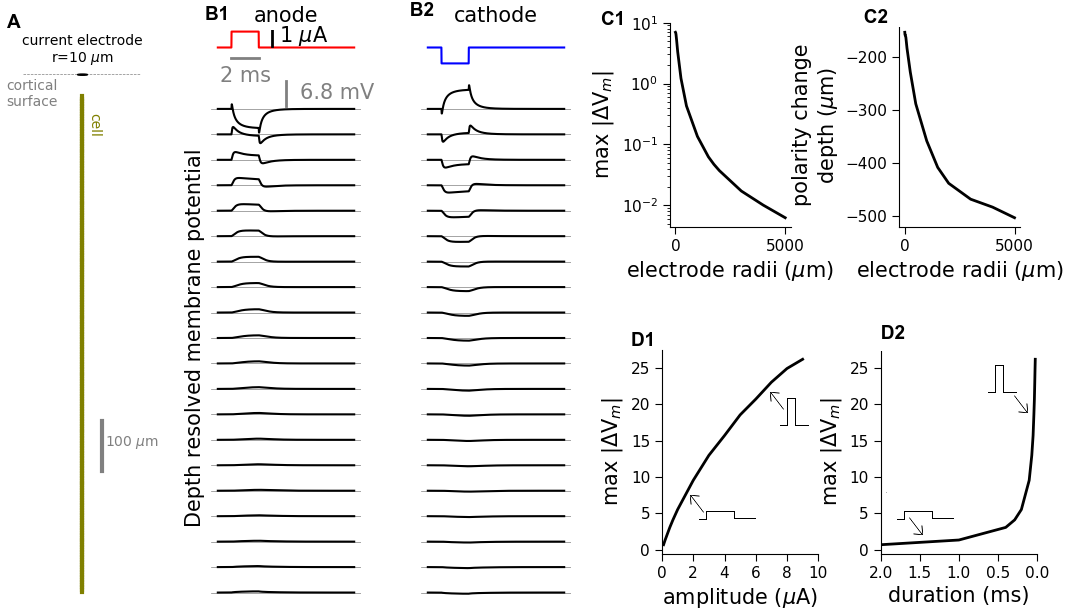
\includegraphics[width=1\textwidth]{Figures/Stim/current_stimulation_example.png}
\end{center}
\caption{\textbf{Illustration of extracellular stimulation (from cortical surface)} 
}
\label{Stim:fig:current_stimulation_example}
\end{figure}

\section{Electrode models for current-carrying electrodes}
\label{Sec:EPI}
In Section~\ref{sec:VC:electrodes} we stated that modelling recording electrodes
was quite easy, but that substantially more complex electrode models might be needed to accurately represent current stimulation electrodes because of electrode polarization
 \cite**{McIntyre2001,Martinsen2008,Joucla2012}.
In essence, the complication stems from that in electronics the electric charge is carried by electrons, while in neural tissue the electric charge is carried by positive and negative ions. For low frequencies, which do not favor capacitive currents, this change of charge carrier can be problematic, resulting in electrode polarization. 
  Modelling electrode polarization effects will often require numerically comprehensive approaches, like the Finite Element Method (FEM) \index{Finite Element Method}\cite**{Buitenweg2003,Moulin2008,Joucla2014,Vermaas2020a}, and/or careful calibration to experimental recordings \cite**{Gabriel1996,Martinsen2008,Miceli2017},
and this topic is not covered here.

Note that for very brief current pulses, the quasi-static approximation might not be applicable \cite**{Bossetti2008,Tracey2011}.